\chapter{Introduction}

\section{Bienvenue dans l’Anthropocène}

\subsection{Le problème du changement climatique}
«~Notre maison brûle, et nous regardons ailleurs » avait joliment déclaré Jacques Chirac en ouverture du IV\up{è} Sommet de la Terre le 2 septembre 2002 à Johannesburg, en Afrique du Sud. Mais la tournure passive est ici trompeuse. La planète Terre est engagée dans une crise écologique sans précédent du fait des actions humaines et de leurs impacts sur l'environnement. Il serait plus exact de dire : nous brûlons notre propre maison. \textit{Homo sapiens} est capable d’apprivoiser le feu, mais il est en même temps \textit{homo demens} \citep{Morin1999}.

Le constat d'une marque visible des activités anthropiques n'est, certes, pas nouveau. Dès 1778, \citeauthor{Buffon1778} notait que «~la face entière de la Terre porte aujourd'hui l'empreinte de la puissance de l'homme~». La nouveauté porte plutôt sur l'ampleur et la vitesse des mutations observées. Depuis 1950, la population a été multipliée par trois, et le PIB a littéralement décuplé : c’est la «~Grande Accélération~».\footnote{Terme apparu en 2005 lors de la conférence de Dahlem sur les relations humain-environnement \citep{costanza2006}}
En l'espace de seulement deux générations, les humains sont devenus une force capable de modeler profondément son environnement à l'échelle mondiale, «~une force tellurique qui change la face de la Terre autant que les éruptions volcaniques~» \citep{Fressoz2013}. 

Mais cette une «~croissance phénoménale du système socio-économique~» \citep{Steffen2004} inquiète. L’humain perturbe les équilibres écologiques et épuise les ressources à sa disposition. Cette année, nous aurons consommé en six mois ce que la planète met un an à produire\footnote{Le jour du dépassement,  «overshooting day~» en anglais, a eu lieu le 2 août en 2017, \url{http://www.overshootday.org/}.}. L’effondrement de la biodiversité et la diminution rapide des effectifs de nombreuses espèces sont tels que les biologistes parlent aujourd’hui de «~sixième extinction de masse~». Les conséquences de l'action humaine sont même déjà observables par les géologues au niveau des sédiments, avec l'accumulation rapide d'aluminium, de béton, de plastiques et de résidus issus de la combustion d'énergie fossiles \citep{Waters2016}. La signature stratigraphique dans les sédiments est suffisamment étendue, claire et distincte pour que le groupe de recherche de la Commission Internationale de Stratigraphie conclue en 2012 : «~l'Holocène est terminée~» \citep{Latour2014}. Nous sommes donc entrés dans une nouvelle époque géologique : l'Anthropocène, dans laquelle l'«Antropos» touche aux limites écologiques et change l'environnement au niveau mondial.\footnote{La date exacte de passage est encore débattue. \citet{Crutzen2000} suggère la fin du XVIII\up{è} siècle, en lien avec l'invention de la machine à vapeur par James Watt et la première révolution industrielle. \citet{Zalasiewicz2014} estiment le début de cette grande accélération au lundi 16 juillet 1945, date du premier essai nucléaire, dans le désert de Mexico. \citet{Steffen2015}  plaident pour 1950, car ils n'observent pas de réelle bouleversement avant cette date : «~the evidence of large-scale shifts in Earth System functioning prior to 1950 is weak~».}

Le phénomène le plus connu de cette «~mutation de notre rapport au monde~» \citep{Latour2015} est sans doute le changement climatique  - ou plutôt les changements climatiques, car les effets sont multiples et divers selon les régions.
Le centre de recherche atmosphérique installé à Mauna Loa, à Hawaï, permet d'observer depuis 1958 une augmentation continue des émissions de CO\textsubscript{2}. Les preuves scientifiques se sont ensuite accumulées pour montrer que la vitesse d'augmentation et le niveau atteint par la concentration de carbone dans l'atmosphère lors des dernières décennies sont sans commune mesure avec ce qu'a connu la Terre dans son histoire, y compris lors des cycles glaciaires/interglaciaires. En 1998, \citet{Mann1998} publiaient un graphique de la températures des 600 dernières années, montrant l'augmentation subite sur la seconde moitié du XX\up{è} siècle, d'où la désormais célèbre forme en «~crosse de hockey~». 
Dans les années suivantes, des carottages en Antarctique permirent de reconstituer les températures et teneurs en CO\textsubscript{2} sur plus de 800 000 ans et de souligner la forte corrélation entre les deux \citep{Petit1999,Luthi2008}.
Dans le graphique \ref{fig:CO2Emissions}, je combine les données récentes de Mauna Loa avec les données historiques issues de l'analyse des glaces antarctiques pour illustrer à quel point la concentration de carbone actuel excède de loin ce qu'à connu la planète puis 800 000 ans, tant en termes de niveau absolu qu'en vitesse d'accumulation. Les taux de CO\textsubscript{2} dans l'atmosphère sont restés compris entre 170 et 300 ppm pendant près d'un milliard d'années -- ce qui inclut plusieurs cycles glaciaires dont la périodicité approche les 40 000 ans; ils dépassent aujourd'hui les 400 ppm, avec une augmentation de presque 100 ppm en seulement un demi-siècle.

\begin{figure}[!ht]
	\centering
	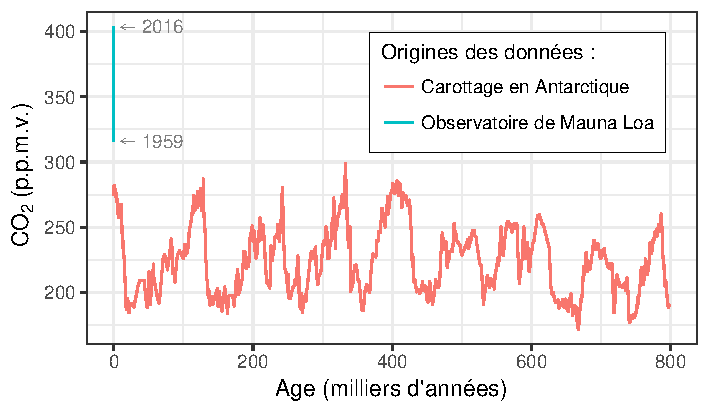
\includegraphics{figures/CO2Emissions.pdf}
	\caption[Concentration de CO\textsubscript{2} dans l'atmosphère]{Concentration de CO\textsubscript{2} dans l'atmosphère \\ Sources : \citet{Luthi2008}, donnée du Dr. Pieter Tans, NOAA/ESRL (\url{www.esrl.noaa.gov/gmd/ccgg/trends/}) du Dr. Ralph Keeling, Scripps Institution of Oceanography (\url{scrippsco2.ucsd.edu/).}}
	\label{fig:CO2Emissions}
\end{figure}

La réalité de ce réchauffement climatique est aujourd’hui «~sans équivoque~» pour la communauté scientifique des climatologues, et l'influence de l'homme sur le système climatique est «~clairement établie~» \citep{IPCC2014}.
A moins de réduire nos émissions de gaz à effet de serre, ce changement climatique va donc s’accentuer, ainsi que ses effets. Et les populations humaines seront directement concernées. La sécurité alimentaire sera menacée du fait d’impacts négatifs sur les récoltes agricoles et la pêche. L’eau sera plus rare dans les régions sèches, menant à une plus forte compétition entre les usages. Les événement extrêmes -- vague de chaleur, précipitations violentes, cyclones --, et leurs conséquences -- inondations, sécheresses et incendies -- pourraient continuer à croitre en fréquence ou en intensité. Les océans vont continuer de s’acidifier et de se réchauffer, avec une hausse globale du niveau des mers. 
Enfin, ces bouleversements frapperont inégalement les populations : les plus démunis sont aussi les plus vulnérables aux effets du changement climatique \citep{IPCC2014}.


\subsection{Les renouvelables, technologies clés pour atténuer les changements climatiques}
Face à ces menaces, l’Accord de Paris, approuvé le 12 décembre 2015, se fixe pour objectif de «~conten[ir] l’élévation de la température moyenne de la planète nettement en dessous de 2 \degree C par rapport aux niveaux préindustriels~». 
Dans cette optique, l’accord rappelle l’importance de cesser l’investissement dans les énergies fossiles, afin de rendre les flux financiers «~compatibles avec un profil d’évolution vers un développement  à faible émission de gaz  à effet de serre~».  Il réaffirme également, dans l’article 4, l’objectif d’atteindre le plus rapidement possible la neutralité carbone : «~les Parties cherchent  à parvenir au plafonnement mondial des émissions de gaz  à effet de serre dans les meilleurs délais ».

Pour prendre la relève des énergies fossiles et atteindre le «~net zéro carbone~» permettant de plafonner les émissions, les renouvelables ont un rôle clé à jouer. Ces nouvelles technologies permettent en effet de continuer à utiliser l’énergie pour nos activités économique, tout en réduisant notre empreinte carbone.
Les énergies renouvelables ne sont pas une panacée, un remède miracle permettant d’atteindre aisément nos objectifs climatiques. Leur déploiement doit s’accompagner d’efforts sur d’autres fronts, notamment sur l’efficacité énergétique, au cœur de la stratégie de l’AIE\footnote{« \textit{there is no realistic, or affordable, energy development strategy that is not led by energy efficiency. For the IEA, it is the first fuel}~» \citep{IEA2016Efficiency}},
et la sobriété énergétique\footnote{L'association négaWatt définit la sobriété énergétique comme le fait de «~réduire à la source la quantité d’énergie nécessaire pour un même service, c’est-à-dire mieux utiliser l’énergie à qualité de vie constante~», \url{https://negawatt.org/La-demarche-negaWatt}}, concept central dans la démarche négaWatt en France\footnote{«~La sobriété et l’efficacité sont les clés de l’inflexion de la demande~»\citep{NegaWatt2017}}, et l'adaptation aux changements climatiques.
Mais ces grandes familles d’action ne sauraient être suffisantes. Même dans une volontariste diminution de la consommation comme le scénario négaWatt, la demande d’énergie ne tend pas vers zéro. Les renouvelables sont donc un levier incontournable de l’action contre les changements climatiques.


\subsection{Deux grands enjeux}
Ma thèse s’attache à étudier deux grands enjeux autour du déploiement des renouvelables : le choix d’une stratégie de long terme, et la question des emplois liés à ces énergies renouvelables.

Le choix de stratégie de déploiement, c’est à la fois la détermination d’un niveau cible et d’une vitesse de développement. Quelle part de renouvelables veut-on dans le mix énergétique, et à quel rythme faut-il les faire entrer dans le système jusqu’à atteindre cette cible ? 
Nous présentons les enjeux de ces questions dans la section \ref{sec:intro_renouvelables}.

La thématique des emplois verts est extrêmement présente dans les débats publics et académiques. Mais le contenu en emploi des renouvelables est-il si élevé, comme cela est souvent avancé ? Et si investir dans les renouvelables plutôt que dans les énergies fossiles crée effectivement de l’emploi, quels sont les mécanismes économiques sous-jacents à ce bilan positif ? Nous présentons l’importance de ces questions dans la section \ref{sec:intro_emploi}.



\section{Quelle stratégie de déploiement des énergies renouvelables ? Application au secteur électrique français}

\label{sec:intro_renouvelables}

\subsection{Points de tension pour établir une stratégie : Inerties, arbitrages temporels et incertitudes}
\subsubsection{De profonds bouleversements}
Le déploiement rapide des renouvelables implique un bouleversement profond des infrastructures énergétiques. Par exemple, dans la production d’électricité, il s’agit de passer d’un système centralisé autour de quelques centrales pilotables et un réseau fonctionnant dans une logique descendante, à un système décentralisé devant des flux variables et multidirectionnels. Il faut donc repenser non seulement les moyens de production, mais aussi tous les réseaux électriques qui les relient.
Même exemple dans les transports : sortir du tout carbone implique de repenser les technologies des véhicules, mais également toute l’infrastructure associée, avec par exemple l’installation de bornes de recharge électrique, des pompes à gaz ou des recharges à hydrogène, selon la technologie choisie du véhicule.
Ces bouleversements impliquent d’importants enjeux financiers. 1,8 mille milliards sont investis chaque année dans les infrastructures énergétiques \citep{IEAWIR2016}. Ces flux doivent être redirigés vers des ressources à faibles émissions. 

L’ampleur des bouleversements en cours et à venir, et des montants en jeu, suscite de nombreux débats. Si l’objectif de décarboner les émissions est aujourd’hui largement partagé, les stratégies pour y parvenir divergent. 

\subsubsection{Arbitrages inter-temporels}
Etablir une stratégie, c’est «~coordonner des actions, de manœuvrer habilement pour atteindre un but~» selon le Larousse. Le but global est ici clair : décarboner les sources d’énergie afin de limiter le réchauffement climatique. Au niveau mondial, l’objectif reste celui de contenir l’élévation de la température moyenne de la planète en dessous de 2\degree C par rapport aux niveaux pré-industriels. Au niveau national, depuis l’Accord de Paris, chaque pays définit ses propres engagements en termes d’émissions\footnote{Les deux objectifs n’étant pas nécessairement compatible : les contributions volontaires cumulées aboutiraient ainsi à un réchauffement proche de 3\degree C}. Se pose alors la question du juste rythme, de la vitesse de cette transition, pour atteindre chaque objectif de la façon la plus «~habile~».

Un point de tension provient de l’attitude à adopter face à l’évolution du coût des énergies. Les coûts des énergies renouvelables diminuent rapidement. L’exemple le plus emblématique est celui des panneaux solaires, dont le coût a été divisé par plus de 4 en moins de sept ans \citep{Lazard2016}. Le coût des éoliennes a également été réduit, de 66\% en sept ans \citep{Lazard2016}. Le facteur quatre a également été observé pour les batteries sur la même durée \citep{McKinsey2017EV}, et est attendu pour l’éolien offshore d’ici 2020 \citep{McKinsey2017Wind}. Faut-il agir au maximum tout de suite, ou lisser l’effort dans le temps pour bénéficier des baisses de coûts ? En effet, plus l’action est progressive, et plus il est possible de bénéficier des progrès de la R\&D et des retours d’expérience, et donc de décarboner à moindre coût.
On voit ici surgir la question des arbitrages inter-temporels. Dans une perspective d’analyse coût-bénéfice, ces arbitrages doivent mettre en regard le coût des émissions supplémentaires face au bénéfice de payer moins cher des technologies qui auront bénéficié de davantage de R\&D ou de plus de retours d’expérience. Cette approche coût-bénéfice est cependant limitée dans le cas du changement climatique, par la difficulté à évaluer les dommages climatiques. Une première raison est l’incertitude liée aux potentiels effets de seuil pour un réchauffement supérieur à 2\degree C par rapport à l'ère pré-industrielle. Une seconde incertitude est liée à la difficulté à évaluer le coût de la part d’une vague de migration climatique, d’une vie humaine ou de la perte d’un écosystème. 
Pour toutes ces raisons, l’approche coût-bénéfice est aujourd’hui de plus en plus délaissée au profit d’une méthode dite de coût-efficacité : il s’agit d’établir la stratégie à moindre coût pour aboutir à un objectif fixé d’avance (les 2\degree C ou les objectifs d’un Etat). L’arbitrage intertemporel repose alors sur la notion de l’actualisation.\footnote{Le choix d’un taux d’actualisation se fonde souvent sur la règle de \citet{Ramsey1928} : $r = \delta + \gamma \cdot g$,
où $r$ est le taux d’actualisation, $\delta$est le taux de préférence pur pour le présent, $g$ est le taux de croissance du revenu individuel, et $\gamma$ est l’élasticité de l’utilité marginale de consommation. \citet{Gollier2011} recommande d’utiliser un taux de 2.5 \% à 3.5 \% pour des horizons inférieurs à 20 ans, et de 1 \% pour des termes au-delà de 100 ans. 
} 

Ainsi présenté, le problème peut paraître simple : en actualisant les prévisions des différents paramètres du problèmes (coût des technologies, demande d’énergie, etc), le choix d’une stratégie revient à un simple problème d’optimisation. 
Mais ce problème est en réalité rendu complexe par la conjonction de deux facteurs : les inerties des systèmes énergétiques, et les fortes incertitudes sur les paramètres clés de la décision.

\subsubsection{Inertie des systèmes énergétiques}
Le premier point concerne la gestion des infrastructures déjà existantes, qu’il s’agisse de moyen de production d’énergie ou de réseaux. Il faut réussir à sortir rapidement de ces énergies carbonées, tout en limitant les pertes économiques importantes qui découleraient d’actifs échoués. Il y a donc toute une dépendance au sentier à prendre en compte. Les choix passés historiques définissent les capacités et les moyens de l’action, d’autant plus que les infrastructures énergétiques s’inscrivent dans la durée. Une centrale à gaz ou à charbon peuvent fonctionner plus de 50 ans \citep{IEA2005}. La durée de vie des réseaux électriques est encore supérieure : les réseaux électriques français ont été installés durant le deuxième quart du XX\up{è} siècle. Ces longues durées de vie induisent une inertie du système dont doit tenir compte toute politique climatique.

\subsubsection{Incertitudes}
Cependant, ces problématiques d’inertie et de d’évolution des coûts sont décuplées par la présence d’incertitudes multiples.
Une première catégorie d’incertitude provient des coûts des technologies futures. La rapide décroissance du coût des énergies renouvelables n’avait pas été anticipée par les experts \citep{Metayer2015}. Cette mauvaise anticipation du passé souligne la fragilité des estimations futures. La rapide baisse des coûts technologiques va-t-elle se poursuivre, ou au contraire finir par atterrir à un niveau stable ? 
Une seconde catégorie d’incertitudes concerne la croissance économique. La crise économique de 2008 et la grande dépression qui s’ensuivit nous rappellent avec force la possibilité d’accident imprévus. Or, l’évolution de cette croissance est importante à double titre : par son impact sur la demande d’énergie, et par son rôle dans l’estimation du taux d’actualisation. 
Une troisième catégorie a trait aux coûts des énergies fossiles. Les rapports alarmants sur le risque d’un pic de pétrole ne manquent pas depuis le célèbre rapport du Club de Rome, \textit{The limit to growth} \citep{Meadows1972}. En 2012, les prix du Brent dépassèrent les 130 \$ par baril, ravivant des inquiétudes sur l’imminence du pic. Mais l’avènement de la fracturation hydraulique et l’arrivée massive sur le marché mondiale du pétrole de schiste américain a fait replonger les prix à des niveaux historiquement bas en 2015. Alors que les prix s’établissaient autour de 110 \$ par baril entre 2011 et 2014, ils se sont effondrés aux alentours de 50 \$ passé 2015. Autant de rebondissements révélateurs de l’incertitude sur les ressources, les techniques d’extraction et \textit{in fine} les prix. 
Des incertitudes techniques similaires existent pour le gaz, comme en témoigne la révolution des gaz de schiste. En outre, le prix du gaz est en partie indexé sur celui du pétrole en Europe, et subi donc ses fluctuations. 

Enfin, il existe une incertitude sur la volonté politique de prendre en compte le changement climatique. Très concrètement, pour l’économiste, cette incertitude prend notamment la forme d’une incertitude sur le prix du CO2 à considérer. Le marché de quotas européen, le SCEQE (plus connu sous l’acronyme anglais de EU ETS), considéré comme un exemple emblématique d’un marché de quota, a ainsi connu de fortes variations. Le prix a dépassé 30 euros la tonne à certains moments, avant de se fixer sous les 10 euros depuis le début de la phase III en 2013. 

Notons bien qu’il s’agit ici d’incertitudes radicales. Ce concept d’incertitude, au sens de \citet{Knight1921}, est à distinguer de celui de risque par l’impossibilité même de prévoir une distribution de probabilité des cas possibles.\footnote{On peut trouver dans la littérature d’autres terminologies équivalentes, et notamment celle d'incertitude profonde (\textit{deep uncertainty})}
«~La différence pratique entre les deux catégories, le risque et l’incertitude, est que, s’agissant de la première, la distribution du résultat parmi un ensemble de cas est connue (soit par le calcul a priori, soit par des statistiques fondées sur les fréquences observées), tandis que ceci n’est pas vrai de l’incertitude en raison de l’impossibilité de regrouper les cas, parce que la situation à traiter présente un degré élevé de singularité~»\citep[p. 233]{Knight1921}.
Il est bien sûr impossible de pouvoir définir avec certitude une distribution de probabilité sur les coûts futurs de renouvelables, le taux de croissance économique, le prix des ressources fossiles ou encore celui du CO2. Nous sommes donc bien dans le cas de l’incertitude radicale. Quelle valeur prendre pour chaque paramètre incertain ? Prendre une unique valeur pour chaque paramètre incertain pour minimiser les coûts reviendrait en quelques sortes à nier l’incertitude. Nous cherchons donc une approche qui prenne à bras-le-corps ces incertitudes, qui les intègre pleinement au problème, mais sans les réduire artificiellement. Comme l’a noté Edgar Morin dans \textit{la Méthode}, “La connaissance progresse en intégrant en elle l'incertitude, non en l'exorcisant” \citep{Morin2008}.
En outre, on voit que face à cette incertitude radicale, différentes options politiques peuvent être également défendables, selon les choix d’un politique, selon ses convictions intimes, ou pour le dire autrement, selon ses probabilités implicites sur les futurs états du monde.  Par exemple, un décidant convaincu que les prix du pétrole vont remonter rapidement voudra accélérer la décarbonation des transports. Et il n’est pas possible de dire qu’il a évidemment tort de faire cette hypothèse – non plus qu’il a évidemment raison. Nous cherchons donc une approche qui ne propose pas nécessairement une unique solution.

Toutes ces incertitudes se combinent avec les questions d’inertie, et cette conjonction rend le problème d’arbitrage intertemporel extrêmement complexe. L’inertie implique d’anticiper l’impact des choix faits, car ceux-ci nous engagent sur plusieurs décennies ; mais l’incertitude empêche d’anticiper parfaitement. Comment, dès lors, déterminer la meilleure stratégie ? Nous tentons de répondre à cette question en nous intéressant plus spécifiquement au cas du déploiement des renouvelables en France.

\subsection{Application au secteur électrique français}
\subsubsection{De l’importance du secteur électrique dans la transition}
Dans ma thèse, j’ai choisi d’étudier la question des inerties et des incertitudes à travers le cas du secteur électrique français. Le secteur électrique est au cœur de la transition énergétique. Il s’agit en effet d’un secteur contribuant largement aux émissions mondiales, tout en présentant des possibilités techniques de substitutions : les centrales à gaz, à charbon et à fuel peuvent être remplacées par des éoliennes, des panneaux solaires ou du biogaz.

La révolution des énergies renouvelables électriques a d’ailleurs déjà commencé. L’année 2015 fut celle d’un record absolu en termes de capacités renouvelables installées au niveau mondial avec 153 GW \citep{InternationalEnergyAgency2016}. L’investissement dans les renouvelables électriques a également atteint un nouveau record, en dépit de la plongée des prix du pétrole : 265,8 milliards de dollars, soit plus du double des investissements dans les centrales à gaz ou à charbon [REN21, Global status report 2016]. 
Si la Chine est passée en tête en termes de capacité installée, l’Europe n’est pas en reste. En termes de production renouvelable électrique par habitant (hors hydraulique), les cinq premiers pays du G20 sont tous européens : Danemark, Allemagne, Suède, Espagne et Portugal \citep[p. 21]{REN212016}. Le Danemark en particulier s’est fixé l’objectif de sortir des renouvelables à l’horizon 2050\footnote{\url{http://denmark.dk/en/green-living/strategies-and-policies/independent-from-fossil-fuels-by-2050/}}, et en 2015, la production des renouvelables représentaient déjà 56 \% de la consommation d'électricité dans le pays\footnote{\url{https://ens.dk/en/press\#/pressreleases/renewables-now-cover-56-procent-of-electricity-consumption-1672848}}. 

\begin{figure}[!ht]
	\centering
	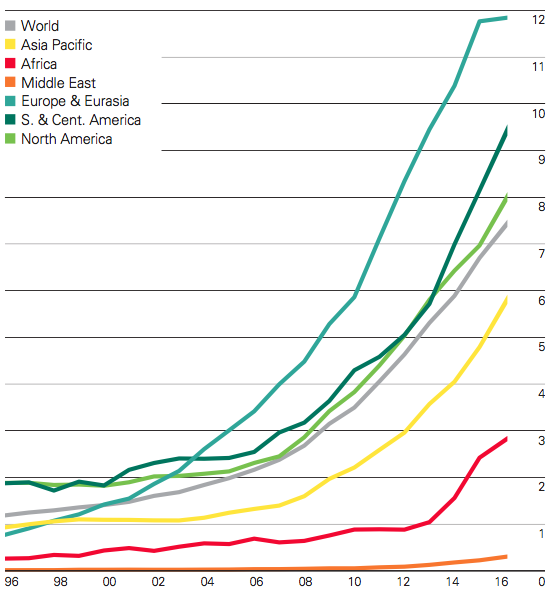
\includegraphics[height=7cm]{figures/BP_ENR_Expansion.png}
	\caption[Expansion of renewable energies in the power sector]{Expansion of renewable energies in the power sector.\\Source: \citet[p. 43]{BP2017}}
\end{figure}

Cette révolution est portée par une volonté politique, avec la mise en place de mécanismes de soutien volontaristes par certains Etats : tarifs d’achat garantis, obligation de quotas, exemption de taxes, appels d’offres, aides à l’investissements, etc.\citep{EuropeanCommission2013}. Et elle est facilitée par une décroissance rapide des coûts des renouvelables. On a ainsi vu s’amorcer une boucle vertueuse, où le soutien politique décroit les coûts, ce qui facilite le soutien politique en retour.

\subsubsection{Contexte politique français}
En France, le mix électrique est déjà largement décarboné du fait de la grande part du nucléaire, qui représentait 72 \% de la production d’électricité en 2016. Avec l’hydraulique à 12 \%, ceci ne laisse qu’une part marginale aux nouvelles énergies renouvelables. L’éolien et le solaire ne comptaient ainsi que pour 5,5 \% \citet{RTE2016}. 
Mais la question du déploiement des renouvelables est sur la table. Avec la Loi sur la Transition Energétique pour la Croissance Verte, la France s’est engagée à porter à 40 \% de la production d’électricité la part des renouvelables d’ici à 2030, et de réduire la part du nucléaire à 50 \% d’ici 2050. Certains doutes existent quant au fait que la France atteigne effectivement ces objectifs, notamment du fait des difficiles compatibilités entre les différents objectifs mentionnés dans la loi - l’IDDRI parle de «~quadrature du cercle~» \citep{Rudinger2017}. Le débat reste donc ouvert.

\begin{figure}[!ht]
	\centering
	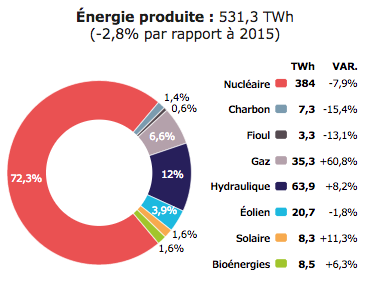
\includegraphics[width=7cm]{figures/RTE_Mix.png}
	\caption[Mix électrique français en 2016]{Mix électrique français en 2016.\\Source: \citet[p. 4]{RTE2016}}
\end{figure}

La situation du parc électrique français présente donc toutes les caractéristiques qui rendent le choix d’une stratégie difficile : la nécessité de faire des choix inter-temporels, en présence d’incertitudes et d’inerties. Inerties et incertitudes sont même particulièrement prégnantes ici avec la technologie nucléaire, au cœur du débat français sur la transition. 

Ce débat a été particulièrement visible lors de la campagne présidentielle de 2017. Une étude diffusée le 13 mars par l’Institut Montaigne présente le nucléaire comme la seule option  «~rationnelle~», et évalue à 217 milliards d’ici 2035 le coût d’une sortie de l’atome.\footnote{\url{http://www.institutmontaigne.org/presidentielle-2017/propositions/benoit-hamon-climat-environnement-et-agriculture-sortir-progressivement-du-nucleaire}} Quatre jours plus tard, une réponse publiée sur le site «~Décrypter l’énergie~» estime au contraire que la sortie du nucléaire représenterait un bénéfice de 24 milliards.\footnote{\url{http://decrypterlenergie.org/fermeture-du-parc-nucleaire-un-cout-largement-surestime-par-linstitut-montaigne}} Le grand écart dans cette bataille de chiffres est surtout révélateur des incertitudes considérables qui entourent la filière. C’est seulement en prenant pleinement acte des nombreuses inconnues qu’il sera possible de faire progresser le dialogue et d’établir une feuille de route pour l’industrie nucléaire française.
Rappelons que l’année a été riche en rebondissements pour la filière nucléaire. Après le démantèlement d’Areva, criblée de dettes, un audit interne à l’entreprise a mis à jour deux anomalies génériques. La première concerne des irrégularités qui «~s’apparent à des falsifications~»\footnote{Selon les propres termes de Pierre-Franck Chevet, président de l'ASN, \url{http://abonnes.lemonde.fr/entreprises/article/2015/07/07/areva-connaissait-de-longue-date-les-anomalies-de-la-cuve-de-l-epr_4674521_1656994.html}} constatées dans plus de 400 dossiers de fabrication de composants. La seconde a trait à des inquiétudes sur la résistance des cuves – élément central et impossible à remplacer - des réacteurs en fonctionnement. Plusieurs centrales nucléaires ont été arrêtées pour inspection cet hiver, allant jusqu’à faire planer le risque d’un possible black-out du système électrique français. Ces anomalies ont touché jusqu’à la cuve de l’EPR de Flamanville, faisant craindre de nouveaux reports pour un chantier qui devait initialement s’achever en 2012, mais ne cesse d’accumuler les retards et les surcoûts. Tous ces éléments ne peuvent que raviver la controverse sur les risques et les coûts réels de cette énergie. 
Or, les centrales nucléaires françaises atteignent aujourd’hui 40 ans, leur durée de vie initialement prévue. La question du futur de l’atome est donc à nouveau sur la table, après quarante ans d’une histoire héritée du premier choc pétrolier. EDF estime pouvoir rénover les réacteurs actuels afin de les prolonger jusqu’à 60 ans, grâce à une opération dite de  «~Grand Carénage~» estimée à 100 milliards d’euros. Faut-il rénover ces centrales ? Ou plutôt, combien de centrales faut-il rénover, et lesquelles ?

\subsection{Méthodologie : Décision robuste et modèle d’optimisation du parc électrique}

\subsubsection{Méthodologie pour déterminer des stratégies robustes}

Face à ces incertitudes, l’approche traditionnelle consiste à choisir a priori un jeu de paramètres pour trouver un optimum, puis à procéder à des tests de sensibilité en faisant varier les paramètres de départ sur les plages plausibles de valeurs. Si le résultat s’avère insensible, autrement dit si l’optimum reste invariant pour toutes les valeurs plausibles de paramètres, alors peut conclure que l’on a trouvé un unique optimum.
Mais que faire si les résultats varient avec différentes valeurs plausibles de paramètres ? 

Une solution de continuité consisterait à donner l’optimum local correspondant à chaque jeu de paramètre. Mais cette approche peut se révéler paralysante pour le décideur, avec une multiplicité d’options possibles, selon des valeurs de paramètres inconnues au moment de la décision.

Face à ces incertitudes radicales, réduire de façon artificielle les incertitudes sur les paramètres, de façon à retrouver un unique optimum, n’est pas une option. Il faut une approche qui admette la possibilité d’aboutir à plusieurs options possibles, à plusieurs stratégies plausibles pour certaines valeurs des paramètres. Cette pluralité de solutions peut permettre de faire le lien avec le débat public : souvent, en présence de fortes incertitudes, plusieurs solutions sont proposées sans qu’il soit possible de déterminer la meilleure avec une absolue certitude. 

L’enjeu est ensuite celui d’une aide à la décision. Il s’agit de simplifier la tâche du décideur face à la multiplicité des paramètres d’entrée du problème. Quels sont les paramètres ou combinaisons de paramètres qui s’avèrent décisifs. Nous chercherons à réduire un problème comportant initialement n paramètres, pour aboutir proposer deux ou trois ensembles de paramètres. Le décideur n’aura alors plus qu’à choisir entre ces ensembles. Mais au final, ce choix nécessite que le décideur fasse un pari sur l’avenir, d’où le choix du titre de l’article qui fait la première partie de cette thèse : le pari nucléaire français (\textit{the French nuclear bet}).

Il peut être également intéressant de délaisser la notion paralysante d’optimum, au profit du concept de trajectoire robuste, définit par \citet{Lempert2006} comme «~une stratégie qui offre une performance satisfaisante dans un grand nombre de futurs plausibles~» - un futur, ou futur état du monde, correspondant à un jeu de paramètres pour notre modèle.
Cette définition générale doit cependant être adaptée à notre objet d’étude particulier. Quel indicateur choisir pour la performance, et qu’est-ce qu’un niveau satisfaisant ?
Pour notre analyse le parc électrique français, nous cherchons assez classiquement à minimiser l'ensemble des coûts, en incluant les coûts en investissement dans la construction du moyen de production, le coût variable de son opération et de sa maintenance, mais aussi les coûts liés au prix du CO\textsubscript{2}. Ce coût total sera donc l’indicateur de performance d’une stratégie.
Une stratégie sera jugée satisfaisante si son coût est assez proche de l’optimum pour le même jeu de paramètres. En utilisant la terminologie de \citet{Savage1950}, on peut introduire le terme de regret, c’est-à-dire de l’écart à l’optimum. Au final, une stratégie robuste est donc celle qui offre un faible regret pour un grand nombre de futurs plausibles.

Pour satisfaire ce cahier des charges que j’ai dessiné, la méthodologie qui m’a paru la plus appropriée est celle présentée par  \citet{Lempert2006}, qu’ils appellent la fabrique de décision robuste (\textit{Robust Decision Making en anglais}, RDM). Cette méthode consiste à appliquer des analyses statistiques sur les résultats d’un grand nombre de scénarios, en mobilisant la notion de regret. Elle s’est initialement développée autour de la thématique du changement climatique, grâce à l’essor des capacités de calculs informatiques. Mais elle peut également être appliquée à une grande variété de cas d’étude : la gestion de l’eau des rivières, l’énergie, la résilience des côtes au changement climatique, etc.\footnote{Une grande liste de projets est visible sur le site \url{https://www.rand.org/topics/robust-decision-making.html?content-type=brief}} Je présente cette méthode plus en détail dans le chapitre \ref{chap:nuclear_bet}.
	
\subsubsection{Cahier des charges pour le modèle d’optimisation}

\textbf{De la nécessité d’aller au-delà du LCOE}

Une métrique est très largement utilisée dans le secteur de l’électricité pour mesurer la compétitivité de différents moyens de production : le coût moyen actualisé de l’électricité, ou plus communément appelée LCOE (\textit{Levelized Cost of Electricity}).
Cet indicateur rassemble en un chiffre unique tous les coûts sur l’ensemble du cycle de vie de la centrale : coûts d’investissement, d’opérations et maintenance, coût du combustible, du financement, du démantèlement, et il les rapporte à la quantité totale d’électricité produite. En bref, le LCOE donne le coût moyen pour produire un mégawatt-heure d’électricité avec un certain moyen de production.

De façon plus formelle, l’\citet{InternationalEnergyAgency2015} définit le LCOE de la façon suivante :
$$LCOE = \frac{\sum_t (Capital_t + O\&M_t + Fuel_t + Carbon_t + D_t) / (1+r)^t}{\sum_t MWh / (1+r)^t}$$
où
\begin{itemize}
	\item MWh = le montant d'électricité produite en MWh, supposé constant ;
	\item $(1+r)^t$ = le facteur d'actualisation;
	\item $Capital_t$ = Ensemble des coûts de capital pour la construction à l'année $t$;
	\item $O\&M_t$ = Coûts d'opération et Maintenance à l'année $t$;
	\item $Fuel_t$  = Coûts de combustible à l'année $t$;
	\item $Carbon_t$ = Coût du carbone à l'année $t$;
	\item $F_t$ = Coût de démantèlement et gestion des déchets à l'année $t$.
\end{itemize}

Cette métrique est utile pour comparer des moyens de productions pilotables. Mais elle n’est plus adaptée pour des moyens de productions variables et non pilotables, comme les énergies éoliennes et solaires. Dès 2011, \citet{Joskow2011a} la dénonçait comme une  «~métrique biasée~» (\textit{flawed metric}). En effet, elle suppose que l’électricité est un produit homogène, et donc régit par la loi d’un prix unique. Mais cette hypothèse est erronée, car elle ignore la variabilité temporelle de la production. Or, la valeur d’un mégawattheure varie selon l’heure du jour et selon la saison : elle est très élevée pendant les heures de pointes, et faible pendant les creux, notamment la nuit. Comme l’électricité ne peut être stockée, il y a bien une hétérogénéité du bien électricité. L’approche par le coût du LCOE ne mesure pas la valeur pour le système, qui est pourtant le bon indicateur : si je produis de l’électricité à faible coût, mais à un moment où personne n’en demande, ma production n’a aucune valeur !

Ce problème de la valeur du moment de la production est renforcé par les phénomènes d’autocorrélation de la production des renouvelables variables. Les panneaux solaires produisent tous à leur maximum vers midi. Ainsi, plus le nombre de panneaux solaires est élevé, plus le prix de l’électricité (représentatif de sa valeur à chaque instant) sera faible à midi. La situation est similaire avec les éoliennes : plus le taux de pénétration des renouvelables est important, plus le prix de marché au moment de leur production diminue, d’où une compétitivité décroissante des renouvelables variables avec le taux de pénétration \citep{Hirth2013}.

\citet{Hirth2016} distinguent par ailleurs deux autres facteurs d’hétérogénéité : le lieu de la production, ce qui inclut notamment la distance au lieu de consommation, et le délai entre le moment du contrat et celui de la livraison. Au total, ces trois sources d’hétérogénéité influent sur la valeur de la production pour le système, ce qui n’est pas inclus dans la notion de LCOE, qui ne traite que des coûts. 
Ces limitations du LCOE justifient l’utilisation d’un modèle intégré du système électrique.

\vspace{1em}
\textbf{Quel modèle choisir ?}

Une grande variété de modèles existe pour l’analyse du mix électrique. Le choix d’un modèle ne peut se faire qu’à travers une analyse précise des besoins liés à la question de recherche.
On peut déjà identifier quelques prérequis :
\begin{itemize}
	\item Je souhaite étudier l’investissement à long terme. Il faut donc que l’investissement soit inclus comme variable endogène au problème. \citet{Petitet2016} distingue trois grandes catégories de modèles : les modèles d’optimisation inter-temporels, les modèles à agents hétérogènes avec des approches par les systèmes dynamiques ; et enfin les modèles micro-économiques de type Bertrand, Cournot ou Stackelberg pour analyser les pouvoirs de marché. 
	\item Je m’intéresse au cas de la France, marché libéralisé mais sous un contrôle strict de la Commission Européenne, et notamment des règles anti-concurrence. En France, c’est plus particulièrement la Commission de Régulation de l’Energie (CRE) qui est en charge de cette mission de surveillance pour le compte de l'Autorité de la Concurrence. Je ne m’intéresse donc pas à aux modèles de concurrence imparfaite et aux pouvoirs de marché. Je me place au contraire dans un cadre de concurrence parfaite, c’est-à-dire que tous les acteurs économiques prennent le prix du marché comme une donnée externe dans leurs décisions, ils ne peuvent l’influer. 
	\item Je cherche à établir ce qui pourrait être la meilleure stratégie plus qu’à anticiper ce que sera l’évolution. Je m’inscris donc dans une perspective plus normative que positive. Les modèles à optimisation intertemporelle me paraissent être plus à même de remplir ce rôle que les approches en simulation. C’est donc sur cette famille de modèles que j’ai arrêté mon choix.
\end{itemize}

\textbf{Hypothèses structurantes}

Dans notre modèle, nous maximisons le profit des producteurs. En effet, d’après le premier théorème du bien-être, cette maximisation conduit à un optimum de Pareto – à condition que les marchés soient complets (sans coût de transaction et avec une information parfaite des agents) et que les firmes soient preneuses de prix. Puisqu’on se place dans une démarche normative, nous supposerons ces deux conditions. 
Nous supposons en outre une parfaite compétition, et une demande d’électricité exogène. Cette dernière hypothèse implique notamment que je ne modélise pas explicitement l'élasticité de la demande, ni à court terme ni à long terme. La littérature empirique donne des résultats variables pour les valeurs de ces élasticités. Pour donner un ordre de grandeur, une méta-analyse de \citet{Labandeira2016} les évalue à 0.23 et 0.67 respectivement. Idéalement, il faudrait aussi détailler les différences entre ménages, industrie électro-intensives et autres industries, voire même les différences saisonnières dans ces élasticités \citep{Fan2011}. Mais dans tous les cas, il est difficile de prévoir quelle seront ces élasticités dans les années et décennies à venir, avec le déploiement des compteurs intelligents Linky en France et la possibilité de faire passer plus de consommateurs vers une tarification en temps réel.
En pratique, l'approximation de demande exogène me semble raisonnable pour un gain très important en termes de temps de calcul. Il s'agit d'ailleurs d'un choix très largement partagé dans la communauté des modélisateurs. D’un point de vue théorique, cette hypothèse permet de poser une équivalence duale entre la maximisation du profit et la minimisation des coûts. 
On ramène donc le problème à celui d’une minimisation des coûts, en sachant que – sous les hypothèses mentionnées – cet objectif est équivalent à maximiser l’utilité.

L’étape suivante consiste à définir les phénomènes que l’on souhaite représenter. Pour notre question de trajectoire optimale, les points suivants m’ont paru essentiels :
\begin{itemize}
	\item Représenter l’ensemble de la trajectoire, de façon continue et cohérente. Il faut une représentation fine des durées de vie des centrales nucléaire, et des prolongations permises par une rénovation.
	\item Représenter l’hydraulique de façon fine, avec notamment un fonctionnement des barrages et des stations de pompage endogène, qui s’adapte au déploiement des renouvelables. La France possède un parc hydraulique qui peut faciliter le déploiement des énergies renouvelables. En effet, la flexibilité de l’hydraulique améliore la valeur des énergies renouvelables variables pour le système électrique \citep{Hirth2016a}.
	\item Avoir une représentation temporelle suffisamment fine pour représenter les variations horaires (avec les pics de demande le matin et le soir), hebdomadaires (avec les baisse de demande le week-end) et saisonnières (avec une production éolienne plus importante en hiver, une production solaire plus forte en été, et une demande d’électricité plus forte en hiver).
\end{itemize}

Pour répondre à tous ces objectifs, j’ai choisi de construire mon propre modèle d’optimisation du parc électrique, que j’ai appelé FLORE (French Linear Optimization for Renewable Expansion). Ce modèle est présenté plus en détail dans le chapitre \ref{chap:nuclear_bet}.
Toute les équations et données du modèle sont disponibles en ligne, dans un esprit de transparence et de partage nécessaires pour la reproductibilité des résultats et d’efficacité du travail de recherche. Je m’inscris pleinement dans cette démarche, recommandée par \citet{Pfenninger2017}, et encore trop absente dans le domaine de l’économie de l’énergie.
Dans le chapitre \ref{chap:nuclear_bet}, je combine la méthodologie RDM et le modèle FLORE afin d’étudier les stratégies robustes de déploiement des renouvelables électriques en France.

\section{L’impact sur l’emploi de la transition énergétique}
\label{sec:intro_emploi}

\subsection{Le choix des emplois liés aux renouvelables comme objet d’étude}
Le débat sur la vitesse de déploiement des énergies renouvelables est doublé dans le débat public et académique d’un débat sur l’emploi. Aujourd’hui, l’emploi est devenu un message clé dans un grand nombre de décisions politiques. 
La question du double dividende emploi est apparue assez tôt dans la littérature avec la prise de conscience du changement climatique. Mais l’enjeu semble aujourd’hui plus fort que jamais, alors que l’essentiel des efforts reste à fournir et que le chômage reste à des niveaux post-crises élevés dans de nombreux pays.

La question de l’emploi nous semble une question de recherche légitime pour deux raisons. La première est l’importance social et humaine de cet enjeu. La littérature sur le déterminant du bonheur souligne l’importance de ne pas trouver un emploi. Il existe un large fossé de bien-être subjectif entre ceux qui possède un emploi, et ceux qui en cherchent sans succès. Comme le souligne le rapport Stiglitz : 
«~Toutes les recherches sur le bien-être subjectif se rejoignent sur un aspect : le coût humain élevé engendré par le chômage. Les chômeurs se disent moins satisfaits de leur vie que les personnes ayant un emploi, même si l'on élimine l'effet de la baisse de revenu~» \citep[p. 166]{Stiglitz2009}.
Et cette importance de l’emploi sur le bien-être est une conclusion stable à travers les générations. C'est par exemple la conclusion des travaux de \citet{Clark2009}, qui étudie des données répétées en coupe :
«~not having a job when you want one is a major source of low well-being. [...] job values have remained fairly stable over time~». 
Etre au chômage augmente même les risques de mortalité et de morbidité, avec une augmentation des taux de suicide et des maladies mortelles \citep{Gerdtham2003}.


La seconde raison est que l’emploi est un levier d’action déterminant pour initier une action politique. Bien plus qu’un épiphénomène ou qu’un simple co-bénéfice, l’emploi est un argument majeur dans le débat sur la transition énergétique. Il semble même presque parfois qu’un renversement s’opère : la transition énergétique ne serait qu’un co-bénéfice d’une politique qui vise avant tout à réduire le chômage. Ainsi en France, deux ans de débats sur la politique énergie-climat ont abouti à une loi intitulée : «~Loi de Transition Energétique pour la croissance verte~»\footnote{Loi n\degree 2015-992 du 17 août 2015
}. La finalité indiquée ici est bien la croissance en premier lieu. Sur son site web, le site du Ministère de l'Ecologie met également en avant que cette loi permettrait de générer «~100 000 emplois~». \footnote{On trouve les annonces suivantes sur le site du Ministère : «~La loi de transition énergétique pour la croissance verte (LTECV) favorise une croissance économique durable et la création d'emploi pérennes et non délocalisables :
\begin{itemize}
	\item elle permet la création de 100 000 emplois à court terme (dont 75 000 dans le secteur de la rénovation énergétique et près de 30 000 dans le secteur des énergies renouvelables) et de plus de 200 000 emplois à l’horizon 2030 ;
	\item le PIB devrait profiter des efforts réalisés à hauteur de 0,8 \% en 2020 et 1,5 \% en 2030.~»
\end{itemize}
\url{https://www.ecologique-solidaire.gouv.fr/loi-transition-energetique-croissance-verte}, accédé le 4 juillet 2017
}
Souligner les effets positifs en termes d’emplois est d’autant plus important que le réchauffement climatique s’apparente à un problème de bien commun. Chaque Etat a intérêt à laisser les autres faire le maximum d’efforts, à jouer les passagers clandestins au maximum. On retrouve formellement le problème du dilemme du prisonnier.
S’il est alors possible de montrer qu’il existe d’importants co-bénéfices à agir de façon coordonnée et coopérative, alors il est possible de sortir de ce dilemme. Il serait alors possible de progresser sur les deux fronts du climat et de l’emploi. Les renouvelables tiendraient alors de la panacée, ce remède à tous les maux. 

On comprend bien alors l’intérêt des chercheurs pour ces deux thématiques. Leur conjugaison est d’ailleurs de plus en plus fréquente dans le domaine académique. On peut le mesurer grâce à la base de données Web of Science, qui agrège les publications de recherche. Une recherche  «~employment AND energy~»\footnote{Recherche effectuée le 12 juillet 2017. Requête exacte : TS=(employment AND energy) AND SU=("Business \& Economics" OR "Environmental Sciences \& Ecology" OR "Energy \& Fuels")} donne une tendance exponentielle du nombre de travaux sur croisant ces deux sujets depuis la crise économique (cf. graphique \ref{fig:webofScience}).
Mais cet intérêt dépasse la sphère académique, et se retrouve également dans le domaine public. En interrogeant la base de données Factiva\footnote{Recherche effectuée le 12 juillet 2017. Requête exacte : "emploi AND énergie"}, qui répertorie les parutions dans la presse française, on peut constater une forte augmentation, commençant un peu plus tôt, dès 2002, avec un pic probablement lié au débat sur la loi de transition énergétique en 2014 (cf. graphique \ref{fig:Factiva}). 


\begin{figure}
	\centering
	\subfloat[Web of Science, résultats pour "employment AND energy"] {
		\makebox[5.5cm][c]{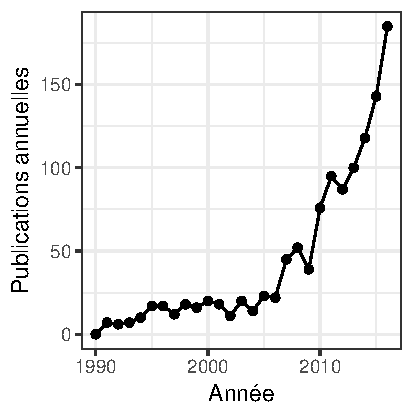
\includegraphics[height=5cm]{figures/EmploymentEnergy.pdf}}
		\label{fig:webofScience}
	} \qquad
	\subfloat[Factiva, résultats pour "emploi AND énergie"][Factiva, résultats pour \\ "emploi AND énergie"]{
		\makebox[6cm][c]{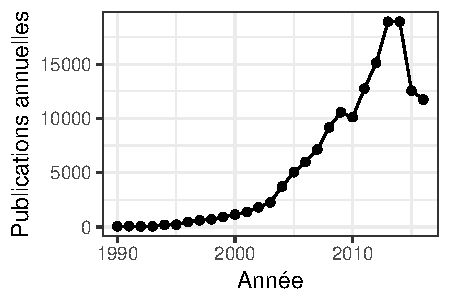
\includegraphics[height=5cm]{figures/Factiva.pdf}}
		\label{fig:Factiva}
	}
\end{figure}

C’est pour ces deux raisons, l’importance social de l’emploi et son potentiel de levier d’action dans la transition énergétique, que j’ai choisi l’emploi dans la transition énergétique comme deuxième thématique de ma thèse.
Ma réflexion a d’abord porté sur la notion de contenu en emploi, souvent utilisé dans les médias, mais également dans les publications académiques. Qu’est-ce que le contenu en emploi ? Est-il plus élevé dans les secteurs de la transition énergétique ? 
Si certains secteurs ont un contenu en emploi plus élevé, alors il serait possible de créer des emplois en réallouant la demande finale vers ceux-ci. Puisqu’il s’agit simplement de réallouer, et non d’augmenter les dépenses, cette mesure peut être particulièrement attractive pour des décideurs au budget contraint. Le contenu en emploi donne une mesure du bilan net de cette réallocation. Mais il reste muet sur les mécanismes économiques sous-jacents. 
Les deux parties suivantes introduisent de façon plus détaillée les enjeux sur ces questions de contenu en emploi et de mécanismes économiques sous-jacents aux créations d’emploi.




\subsection{Le contenu en emploi des énergies renouvelables}

\subsubsection{Contexte}
L’avantage des renouvelables en termes d’emploi est souvent présenté comme découlant d'une raison très simple : les renouvelables auraient un contenu en emploi plus élevé. Par exemple, selon le réseau Sortir du Nucléaire, «~les renouvelables créent quinze fois plus d’emplois que le nucléaire~» \citep{Les7ventsduCotentin2009}. Greenpeace met en avant que cet avantage est dû au fait qu’il s’agit d’emploi «~de proximité~», «~non délocalisables~» \citep{Greenpeace2011}. Favoriser l’essor des renouvelables au détriment des énergies fossiles ou fissiles permettrait donc de générer de nombreux emplois.

Mais la simplicité de ce message à vocation politique cache une complexité d’un autre ordre pour l’économiste. 
La première concerne la définition même de contenu en emploi. Il existe en effet un flou important quant à l’unité de mesure : s’agit-il du nombre d’emploi par unité de puissance installée (kW) ? par unité d’énergie produite (kWh) ? par euro investi ou dépensé ? En pratique, ces différentes métriques coexistent dans la littérature académique : \citet{Cameron2015} observent des données en emploi par capacité installée, \citet{Quirion2013} des emplois par euro dépensé, \citet{Wei2010} par unité d’énergie produite. Mais elles sont-elles équivalentes en termes de résultats ? Quelle serait la meilleure métrique ?
Une seconde difficulté provient de l’articulation de cette notion avec d’autres éléments du débat public. L’accent est parfois mis sur le fait que les renouvelables ont un caractère local, qu’ils permettent de réduire les importations de gaz ou de charbon. Ils sont également présentés comme étant intensif en travail, plutôt qu’en capital. Quels liens établir entre ces arguments et la notion de contenu en emploi ?
Il faut déjà distinguer les contenus en emploi bruts et nets. Les deux sont importants : le brut pour le local, le net pour le global. Mais nous nous intéressons ici à l’effet net sur l’emploi. Or, l'éolien et le solaire ont commencé à se développer avant d’être compétitif, grâce à des subventions. Mais ces subventions doivent être financées, \textit{in fine} au moyen d’autres taxes et potentiellement de réduction d’emplois dans d’autres secteurs. Comment prendre en compte ces effets indirects des subventions dans la mesure du contenu en emploi, afin de mesurer un impact net ?

\subsubsection{Question de recherche}
Ces interrogations m’ont amené à vouloir décomposer le contenu en emploi. Pourquoi ce contenu en emploi est-il plus élevé dans certaines branches ? Est-ce du fait d’importations plus faibles, d’une plus grande part du travail dans la valeur ajoutée, ou d’autres facteurs ?  Quels sont les facteurs prépondérants expliquant les divergences d’une branche à l’autre ?

Au-delà de ce travail purement descriptif et explicatif, nous espérons pouvoir obtenir une connaissance permettant l’action. Les conséquences sont en effet très différentes si le contenu en emploi est élevé du fait d’importations faibles, ou de salaires faibles. Dans un cas, on relocalise la production et la valeur ajoutée, et donc les emplois. Il s’agit d’une politique économique au détriment de nos partenaires commerciaux ; dans l’autre, on baisse les salaires pour partager le travail,  «~gagner moins pour travailler tous~», en quelque sorte. Les conséquences économiques, politiques et sociales sont donc très différentes d’une situation à l’autre.

Enfin, nous espérons pouvoir dégager des secteurs favorables à la transition énergétique et sociale, en croisant ce contenu en emploi avec un contenu en émissions de gaz à effet de serre (GES). Si on peut déterminer des secteurs qui soient à la fois fortement créateurs d’emplois et faiblement émetteurs de GES, alors on aura trouvé ce double dividende emploi, cette politique sans regret. 

\subsubsection{Méthodologie [Input-Output]}
Pour ce travail, nous nous appuyons sur la méthodologie Input-Output (IO). 
C’est une méthodologie couramment employée pour parler de contenu en emploi. Elle est très utile pour un travail descriptif.
Cependant, cette méthodologie doit être utilisée avec précaution dans son aspect prédictif, si on envisage une variation de la demande finale. En effet, l’input-output est un cas particulier de CGE, avec quelques hypothèses fortes : prix fixes (les modèles IO sont d’ailleurs parfois appelés modèles à prix fixes), coefficient constant dans la fonction de production avec une fonction de production dite de Leontief, taux d’importations constants pour chaque secteur, consommation finale des ménages, des administrations publiques exogènes, tout comme la demande finale. Ces définitions exogènes passent sous silence le financement, par exemple en cas d’augmentation des investissements, et doivent donc s'inscrire dans le cadre de scénarios précis. Une autre hypothèse forte est l'assimilation du marginal au moyen : en considérant que chaque branche économique produit un bien homogène, toute la variabilité interne à la branche est ignorée.

En pratique, ces hypothèses restreignent le domaine d’utilisation du modèle IO. Il faut regarder des échelles de temps relativement courtes, afin que les fonctions de production n’évoluent pas trop, ce qui permet de ne pas s’écarter trop e l’hypothèse des coefficients fixes, voire de celle des prix fixes. Il faut également considérer des changements qui ne soient pas des bouleversements, pour ne pas violer l’hypothèse que le marginal est égal au moyen.
Enfin, pour prendre en compte les questions de financements des investissements, et donc bien mesurer un effet net (et non pas un effet brut), on peut travailler à budget constant.

Avec ces précautions méthodologiques, les modèles IO continuent à être utilisés et des travaux publiés par la communauté des chercheurs. On trouve des analyses en de l'impact sur l'emploi de la transition énergétique, mais aussi des analyses sur les émissions des GES ou sur les chaînes de valeur \citep{Timmer2014}.
Au global, les modèles input-output sont de plus en plus utilisés, comme le montre une interrogation de la base de données Web of Science : une recherche sur  "input-output"\footnote{Recherche effectuée la 17 juillet 2017. Requête exacte : «TS=input-output AND SU=("Business \& Economics" OR "Environmental Sciences \& Ecology" OR "Energy \& Fuels")"} montre une augmentation très rapide du nombre de modèle IO utilisés (cf. graphiques \ref{fig:WoS_IO}). Une recherche sur  "input-output AND employment"\footnote{Recherche effectuée le 17 juillet 2017. Requête exacte : «TS=(input-output AND employment) AND SU=("Business \& Economics" OR "Environmental Sciences \& Ecology" OR "Energy \& Fuels")"} montre également une augmentation (cf. graphique \ref{fig:WoS_IO_Environement}). 

\begin{figure}
	\centering
	\subfloat[Web of Science, Résultats pour "Input-Ouput"] {
		\makebox[5cm][c]
			{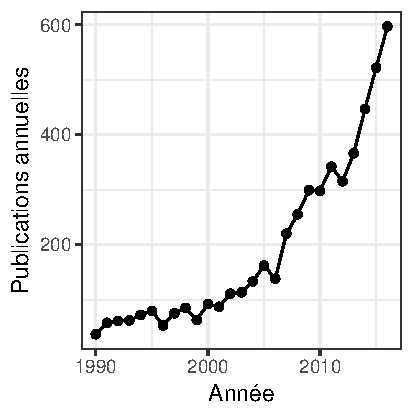
\includegraphics[height=5cm]{figures/WoS_IO.pdf}}
		\label{fig:WoS_IO}
	} \qquad
	\subfloat[Web of Science, résultats pour "Input-Output AND employment"] {
		\makebox[5cm][c]{
			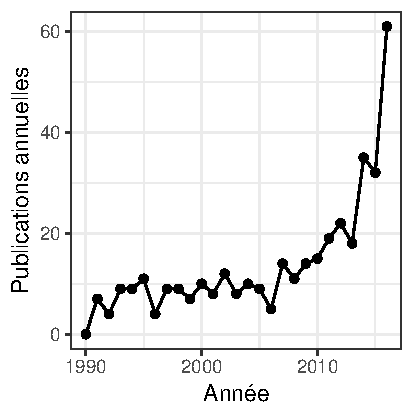
\includegraphics[height=5cm]{figures/WoS_IOEmployment.pdf}
		}
		\label{fig:WoS_IO_Environement}
	}
\end{figure}






\subsection{Emplois verts et réallocation de la demande finale : mécanismes et résultats robustes}
\subsubsection{Contexte}
La partie précédente cherchait à mieux cerner la définition du contenu en emploi, et les causes de ses variations. J’ai montré que certaines branches ont un contenu en emploi plus élevé. 
La partie suivante prolonge cette réflexion sur les emplois verts, avec une réflexion sur l’importance des modèles utilisés dans le résultat. 

De par l'importance politiques de la thématique de l''emploi, des nombreuses études cherchent à quantifier l'impact sur l'emploi d'une transition énergétique. Les résultats de la littérature sont cependant partagés : certains y voient un effet positif, d’autres un effet négatif.

\subsubsection{Question de recherche}
Cependant, il est difficile de dégager des conclusions robustes de ces travaux. La première raison est la pluralité des scénarios étudiés. Il y a une grande variabilité dans les pays, les années, les technologies étudiés ; dans les hypothèses faites (exportations des technologies par exemple).
Mais une autre raison est la diversité des modèles utilisés : IO, CGE, économétrique…

Cette diversité de résultats, de scénarios et de modèle appelle plusieurs questions. Quels sont les résultats robustes d’un modèle à l’autre, et ceux qui divergent ? Et au-delà des résultats, quels sont les mécanismes qui amènent à de la création d’emploi ? L’idée est, au-delà des modèles et des résultats quantitatifs, de pouvoir développer une compréhension des phénomènes économiques à l’œuvre. 

J’ai concentré mon travail sur la comparaison entre les deux types de modèles les plus utilisés pour les analyses en emploi de la transition énergétique : IO et CGE. Ce choix de comparer IO et CGE permet en outre de développer la réflexion sur le modèle IO utilisé dans la partie précédente.

Par ailleurs, j’ai choisi de me concentrer sur l’analyse d’un type de scénarios bien précis : une réallocation des investissements. L’idée est de regarder si investir dans certains secteurs de la transition énergétique permet de générer des emplois. Cette question me paraît pertinente car elle répond à l’impératif d’investissement dans les énergies renouvelables pour décarboner nos modes de production, tout en intégrant la contrainte budgétaire pour les Etats.

\subsubsection{Méthodologie [IO et CGE]}
Je commence par mettre en évidence trois mécanismes principaux de création d’emplois dans un modèle IO : salaires, part du travail dans la valeur ajoutée et taux d’importations. Ces éléments ont un côté intuitif qui résonne dans le débat public. Mais sont-ils confirmés dans un cadre d’équilibre général ?
Pour tenter de répondre à cette question, je développe pour chaque mécanisme un modèle simple d’équilibre général, permettant une comparaison avec le modèle IO. 
Ensuite, je développe et j’utilise un modèle CGE complet, que je compare à un modèle IO. 
Le modèle utilisé est le plus standard possible : il est présenté dans un manuel de macroéconomie \citep{Hosoe2010}, et publié sur le site officiel de la communauté de modélisateurs GAMS. Ce choix est fait pour que les résultats et les mécanismes observés soient les plus généraux et les plus transparents possibles. En outre, l'utilisation d'un CGE permet d'obtenir une estimation quantitative d’une politique énergétique et climatique. En particulier, j'étudie une politique réduisant l’investissement dans les énergies fossiles et augmentant l’investissement dans les énergies renouvelables. 


%%%%%%%%%%%%%%%%%%%%%%%%%%%%

\section{Plan de la thèse}

Le plan de ma thèse s'articule autour de ces deux grands enjeux : le choix d'une stratégie de long terme et la question de l'emploi.
Il en résulte deux grandes parties pouvant être lues de manière relativement autonome.

La première partie correspondant au chapitre \ref{chap:nuclear_bet}. A travers le cas d'un secteur électrique français et la question de la prolongation des centrales nucléaires, j'étudie les questions d'incertitude et d'inertie en appliquant la méthodologie RDM à un modèle d'optimisation du parc électrique construit spécifiquement pour cette question : FLORE. 
Après une introduction du contexte, j'insiste d'abord sur l'amplitude des incertitudes existantes. Je présente ensuite le modèle FLORE et la méthodologie RDM. 
L'application conjointe des deux permet d'aboutir à des recommandations concrètes pour la politique publique, en lien les débats actuels sur le nombre de réacteurs à rénover. Je conclus en proposant de nouvelles stratégies pour le déploiement des renouvelables, qui me paraissent meilleures que les scénarios de référence proposés pendant le Débat National sur la Transition Energétique.

La seconde partie est composée des chapitres \ref{chap:TE_Emploi} et \ref{chap:mechanisms}. J'y explore les impacts sur l'emploi de la transition énergétique. La perspective est ici macroéconomique, et non plus sectorielle comme dans la partie précédente.
Dans le chapitre \ref{chap:TE_Emploi}, je m'intéresse plus particulièrement à la notion de contenu en emploi des différents secteurs économiques. En croisant l'intensité en emploi et l'intensité en émissions de GES, à l'aide d'une méthode de type Input-Output, je donne une vision des secteurs qui semblent les plus favorables à une transition écologique et sociale. Je propose ensuite une méthode nouvelle pour décomposer le contenu en emploi, afin de mieux en saisir ses composantes et leur importance relative : taux d'importations, part du travail dans la valeur ajoutée, niveaux des salaires ou montant des taxes et subventions. Ma décomposition montre que les taxes induisent un effet distorsif dans cette métrique, et permet de corriger cet effet. Elle aide en outre à mieux cerner les effets à l'\oe{}uvre dans les modèles macro-économiques.

Je poursuis cette réflexion sur les causes et les mécanismes économiques présidant à la création d'emploi dans le chapitre \ref{chap:mechanisms}. J'étudie spécifiquement le cas d'une réallocation de l'investissement, en mobilisant des modèles de type CGE et Input-Output. Je montre que trois facteurs sont à la source d'une évolution de l'emploi : le taux d'importations, la part du travail dans la valeur ajoutée et le niveau de salaires. Cette mise en évidence dans les équations des modèles fait donc le lien avec la décomposition descriptive du chapitre précédent. Mais cette partie met aussi en évidence un effet plus ambigu des importations : encourager les secteurs faiblement importateurs a des effets très positifs en Input-Output, et beaucoup moins dans les modèles CGE. Enfin, je réalise l'évaluation quantitative de deux politiques publiques : investir dans l'isolation des bâtiments et les panneaux solaires PV privés. Je montre que dans ces deux cas, l'impact sur l'emploi est positif grâce à la forte part de travail dans la valeur ajoutée et le faible niveau de salaire, et que ce résultat est robuste à travers les deux familles de modèles. 

Pour finir, je présente les conclusions de ma thèse dans le chapitre \ref{chap:conclusion}. Je replace mes résultats dans une perspective plus large, avant d'ouvrir des pistes sur les possibles améliorations et recherches futures.





